\documentclass[10pt,letterpaper]{article}
\usepackage{neverhuman-brief-style}

\renewcommand{\briefrunningtitle}{Technical \& Latency Brief}
\title{NEVERHUMAN Pre-Incision POAF Technical Brief}
\author{NEVERHUMAN Research \& HonorHealth Heart Care}

\begin{document}
\thispagestyle{briefpage1}

\briefmasthead{Technical \& Systems Brief \textbar{} For CTOs, VPs of Engineering \& ML Architects}%
  {Accuracy Meets Real-Time Latency Across 1,091 U.S.\ Hospitals}%
  {Head-to-head national benchmark of \textbf{Google TabFM v1.0.0}, \textbf{NVIDIA KumoTabular-Large v2}, \textbf{PriorLabs TabPFN-3.5}, \textbf{CatBoost}, and \textbf{AutoGluon 1.5} (all binary) vs.\ \textbf{NEVERHUMAN} across strictly unseen and seen hospitals --- including full train/inference profiling.}

% ---- 4 KPI Cards ------------------------------------------------------------
\noindent
\begin{minipage}[t]{0.238\textwidth}\vspace{0pt}
\kpicard{accent}{0.6767 / 0.6916}{Unseen / Seen 208}{NEVERHUMAN ranks \textbf{\#1 at 50k} in both unseen (74 hosp) \& native site-aware seen (1,086 hosp) splits.}
\end{minipage}\hfill
\begin{minipage}[t]{0.238\textwidth}\vspace{0pt}
\kpicard{navy}{+21.8 to +55.3*}{Unseen Margin (bps)}{Beats AutoGluon (+21.8*), CB (+24.5*), TabPFN (+29.2*), Kumo (+52.0*), TabFM (+55.3*); all CIs $>0$.}
\end{minipage}\hfill
\begin{minipage}[t]{0.238\textwidth}\vspace{0pt}
\kpicard{teal}{4.11\,s / 45.2\,ms}{Batch / 1-Pt Infer}{\textbf{0.193\,ms/pt} batch across 21,241 cases; \textbf{0.53\,GB} VRAM; \textbf{19.7\x{}--323\x{} faster} than AutoGluon \& TFMs.}
\end{minipage}\hfill
\begin{minipage}[t]{0.238\textwidth}\vspace{0pt}
\kpicard{blue}{21.5\,min Train}{End-to-End Offline}{28\% faster training than AutoGluon \tcli{best\_quality} (30.0\,min, 10.1\,GB disk) with higher unseen \& seen AUC.}
\end{minipage}

\vspace{4.5pt}

% ---- Speed Showcase Figure Card ---------------------------------------------
\begin{tcolorbox}[enhanced,colback=white,colframe=hair,boxrule=0.5pt,arc=2.5pt,
  left=6pt,right=6pt,top=5pt,bottom=4.5pt]
  {\ftitlefont Training Wall-Clock, Per-Patient Scoring Speed \& Accuracy-vs-Speed Pareto Across All 6 Models}\par
  \vspace{2.5pt}
  \centering
  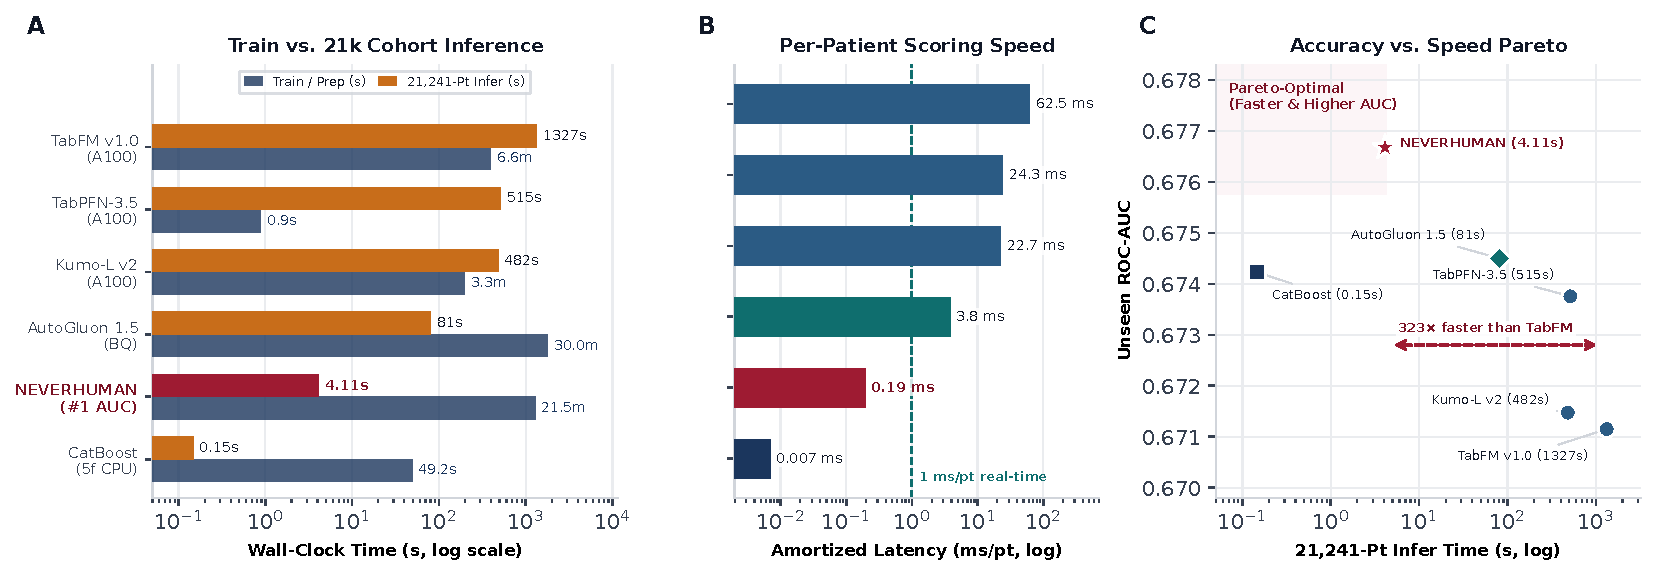
\includegraphics[width=0.99\linewidth]{fig_timing.pdf}
  \vspace{-2pt}
  {\raggedright\sffamily\fontsize{6.2}{7.7}\selectfont\color{sub}\textbf{Systems takeaway:} In-context foundation models (TabPFN-3.5, Kumo-L, TabFM) must attend over 10k--50k training rows at prediction time (482--1,327\,s on A100; 12--41\,GB reserved VRAM). AutoGluon \tcli{best\_quality} serializes 10.1\,GB of models and incurs 81.0\,s batch / 28.5\,s single-patient latency. NEVERHUMAN sits alone in the top-left Pareto optimum: \textbf{4.11\,s} batch (0.19\,ms/pt, 0.53\,GB VRAM) and highest AUC.\par}
\end{tcolorbox}

\vspace{4.5pt}

% ---- Two-Column Engineering Deep Dive ---------------------------------------
\noindent
\begin{minipage}[t]{0.486\textwidth}
  \vspace{0pt}
  \colheading{Zero-Leakage Contract \& Dual-Regime Splits}
  {\fontsize{7.85}{9.7}\selectfont
  Every model consumes identical \textbf{207 raw pre-incision STS variables} (638 $\to$ 207 schema audit purging 7 early-column post-op duration leaks: \tcli{LOS}, \tcli{PLOS}, \tcli{ORDuration}, etc.) and skip-logic reconstructed outcomes (\textbf{367,695 labeled cases}, 24.30\% POAF). Active Python audit hooks block sealed test-label access during training.

  \vspace{2.2pt}
  \textbf{Two controlled 50k $\to$ 21,241 splits:} (1) \textbf{Unseen Hospitals} (74 anticlustered holdout centers, 0.0\% overlap, $\mathrm{Max}|\mathrm{SMD}|{=}0.103$); and (2) \textbf{Seen Hospitals} (all 1,091 centers represented in train, 1,086 test centers, 100.0\% overlap), tested both on 207 raw features and with strictly train-only Empirical-Bayes hospital priors (\tcli{site208} / +EB).
  }
\end{minipage}\hfill
\begin{minipage}[t]{0.486\textwidth}
  \vspace{0pt}
  \colheading{Why Seen-Hospital Overlap Distorts Benchmarks}
  {\fontsize{7.85}{9.7}\selectfont
  Naive calendar-2017 holdouts share \textbf{99.5\%} of hospitals with training, hiding a \textbf{$-$1.99 AUC-point} unseen drop (0.6778 $\to$ 0.6579). On our controlled 100\% Seen split, hospital overlap alone inflates 207-raw AUCs by \textbf{+28--64\,bps} even with zero site IDs---twice as large for tabular foundation models (+49--64\,bps) as for NEVERHUMAN (+28\,bps).

  \vspace{2.2pt}
  Explicit train-only hospital priors lift every 50k model by \textbf{+179--213\,bps} into \textbf{0.6966--0.6986} (and 346k CatBoost to \textbf{0.7014}). Under native 50k \tcli{site208} training, \textbf{NEVERHUMAN leads at 0.6916} (+24.1*\,bps vs.\ AutoGluon \tcli{site208}; +29.0*\,bps vs.\ CatBoost \tcli{site208}).
  }
\end{minipage}

% ==================== PAGE 2 =================================================
\clearpage
\thispagestyle{briefpage2}

\briefsection{01}{Full 6-Model Accuracy, Latency \& Compute Matrix ($N{=}21{,}241$ Natural-Prior Holdouts)}

{\noindent\sffamily\fontsize{6.55}{8.0}\selectfont\color{sub}Identical 50,000-patient 5-fold hospital-grouped cohorts (strictly 207 raw pre-incision variables; AutoGluon enforced via \tcli{groups="cv\_fold"}). Uniform fold-OOF Platt calibration + dev-only Bayes shift (\m 1.1365). 5,000-draw whole-hospital cluster 95\% CIs (seed 42); * strictly excludes zero.\par}

\vspace{2.2pt}
\noindent
{\fontsize{6.95}{8.55}\selectfont\setlength{\tabcolsep}{2.4pt}
\begin{tabularx}{\textwidth}{@{}Y R{1.00cm} R{2.30cm} R{0.92cm} R{0.92cm} R{1.10cm} R{1.12cm} R{1.05cm} R{1.35cm}@{}}
\toprule
\thd{Model (50k Parity Unless Noted)} & \thd{Unseen} & \thd{NEVERHUMAN $\Delta$ Unseen} & \thd{Seen 207} & \thd{Seen 208} & \thd{Seen +EB346k} & \thd{Train / Prep} & \thd{21k Infer} & \thd{1-Pt / VRAM} \\
\midrule
\rowcolor{accenttint}
\textbf{NEVERHUMAN (Proprietary)} & \textbf{0.6767} & \textbf{\#1 @ 50k (0.0072 ECE)} & \textbf{0.6794} & \textbf{0.6916} & \textbf{0.6974} & \textbf{21.5\,m} & \textbf{4.11\,s} & \textbf{45.2\,ms / 0.5\,GB} \\
AutoGluon 1.5 (\tcli{best\_quality}) & 0.6745 & \textbf{+21.8 [+7.0, +36.5]*} & 0.6790 & 0.6891 & 0.6974 & 30.0\,m & 80.99\,s & 28.5\,s / 10.1\,GB* \\
CatBoost (5-fold binary) & 0.6742 & \textbf{+24.5 [+7.2, +42.2]*} & 0.6777 & 0.6886 & 0.6966 & 0.8\,m & 0.15\,s & 3.0\,ms / CPU \\
PriorLabs TabPFN-3.5 (50k nat.) & 0.6738 & \textbf{+29.2 [+8.2, +53.5]*} & 0.6795 & --- & 0.6982 & 0.9\,s & 515.3\,s & In-ctx / 7.7\,GB \\
NVIDIA KumoTabular-Large v2 & 0.6715 & \textbf{+52.0 [+21.6, +83.3]*} & 0.6764 & --- & 0.6977 & 3.3\,m & 481.7\,s & In-ctx / 6.8\,GB \\
Google TabFM v1.0.0 & 0.6712 & \textbf{+55.3 [+28.6, +81.5]*} & 0.6775 & --- & 0.6986 & 6.6\,m & 1,326.7\,s & In-ctx / 22.1\,GB \\
\midrule
\textit{Mariscalco POAF Proxy} & \textit{0.6190} & \textit{\textbf{+577.0 [+495.6, +656.9]*}} & \textit{0.6276} & \textit{---} & \textit{---} & \textit{---} & \textit{$<$0.01\,s} & \textit{Bedside rule} \\
\textit{7\x{} Full-Registry CatBoost (346k)} & \textit{0.6773} & \textit{\m 6.4 [\m 23.0, +10.5]} & \textit{0.6831} & \textit{\textbf{0.7014}} & \textit{---} & \textit{6.2\,m} & \textit{0.30\,s} & \textit{CPU ref} \\
\bottomrule
\end{tabularx}}
\vspace{1.2pt}
{\noindent\sffamily\fontsize{6.0}{7.4}\selectfont\color{sub}*AutoGluon footprint reports serialized disk size (10.1\,GB unseen; 9.9--11.2\,GB across splits); seen raw207 batch infer 4.80\,s (915\,ms 1-pt), \tcli{site208} batch infer 37.78\,s (23.7\,s 1-pt). TFM GPU figures reflect NVIDIA A100-40GB allocated VRAM (reserved: 12.0--40.8\,GB). Literature PROBAST external median: \textbf{0.61} (Table 5 in manuscripts).\par}

\vspace{4.0pt}

\noindent
\begin{minipage}[t]{0.486\textwidth}
  \vspace{0pt}
  \briefsection{02}{Statistical Rigor \& Deployment Economics}
  {\fontsize{7.65}{9.5}\selectfont
  \textbf{Cluster-confirmed unseen superiority:} Every 74-hospital cluster 95\% CI for NEVERHUMAN versus all five binary alternatives strictly clears zero ($P{>}0 = 0.997$--$1.000$). On unseen average precision (0.3777 vs.\ 0.3776) and ECE (0.0072 vs.\ 0.0076), 50k NEVERHUMAN even edges the $7\times$ 346k CatBoost registry model while closing \textbf{79.2\%} of its AUC gap.

  \vspace{2.2pt}
  \textbf{Pareto latency advantage:} NEVERHUMAN delivers sub-millisecond amortized scoring (\textbf{0.193\,ms/pt}) and \textbf{45.2\,ms} single-patient bedside response using \textbf{0.53\,GB} VRAM---running \textbf{19.7\x{} faster} than AutoGluon batch (\textbf{630\x{} faster} bedside), \textbf{117\x{} faster} than Kumo, \textbf{125\x{} faster} than TabPFN-3.5, and \textbf{323\x{} faster} than TabFM.
  }

  \vspace{3.0pt}
  \briefsection{03}{FPR Reduction, U.S./Global Impact \& Literature}
  {\fontsize{7.6}{9.45}\selectfont
  \begin{itemize}[leftmargin=1.12em,itemsep=1.5pt,topsep=1.0pt]
    \item \textbf{Lowest FPR (70\% / 80\% Sens):} \textbf{44.10\% / 55.54\%} unseen (41.22\% seen \tcli{site208})---sparing \textbf{490--1,798 U.S.} (\textbf{2,448--8,992 global}) patients/yr vs.\ AI baselines \& \textbf{48,755 U.S.} vs.\ POAF score.
    \item \textbf{Modeled Impact (200k U.S.\ / 1M Global):} Top-25\% PALACS targeting models \textbf{8,758 U.S.} (\textbf{43,790 global}) POAF cases prevented/yr, \textbf{\$88--131M/yr} U.S.\ savings, and \textbf{30--60 U.S.} (\textbf{149--298 global}) conservative operative deaths averted/yr (STS POAF mortality 2.78\% vs.\ 1.42\%).
    \item \textbf{Literature Frontier:} Published AUCs $>0.72$ use post-op/ICU fields, valve cohorts, or waveforms; 0.677--0.701 defines the true pre-incision STS frontier (PROBAST external median 0.61; Table 5).
  \end{itemize}
  }
\end{minipage}\hfill
\begin{minipage}[t]{0.486\textwidth}
  \vspace{0pt}
  \briefsection{04}{Reproducible Audit \& Verification CLI}
  \begin{codecard}{Zero-Trust Compliance \& Build Verification}
{\color{codecomment}\# 1. Deterministically rebuild BOTH clinical journal PDFs:}\\
make -C docs/nejm\_ai -B\\
make -C docs/npj\_digital\_medicine -B\\[2.5pt]
{\color{codecomment}\# 2. Rebuild \& verify 2-page CEO \& CTO executive briefs:}\\
bash docs/briefs/scripts/build\_briefs.sh\\
bash docs/briefs/scripts/build\_briefs.sh --check\\[2.5pt]
{\color{codecomment}\# 3. Run automated compliance, link \& privacy audit:}\\
python3 scripts/41\_audit\_ip\_clean\_publication.py \\
  --nejm-dir docs/nejm\_ai \\
  --npj-dir docs/npj\_digital\_medicine \\
  --scan-dirs docs reports README.md
  \end{codecard}

  \vspace{2.5pt}
  \begin{govbox}{Technical Boundaries \& Governance}
    \begin{itemize}[leftmargin=1.10em,itemsep=1.5pt,topsep=1.2pt]
      \item \textbf{Proprietary IP protection:} NEVERHUMAN's internal training methods and model weights remain proprietary; every evaluation split, baseline configuration, calibration rule, and timing receipt is transparently archived.
      \item \textbf{Retrospective selection bound:} Multi-model benchmarking requires prospective confirmation of frozen deployment interfaces on post-2017 STS ACSD v4.20+ cohorts.
      \item \textbf{Modality ceiling:} Pushing cold-start unseen discrimination past 0.70 will require raw 12-lead ECG waveforms or left-atrial imaging absent from STS v2.81.
    \end{itemize}
  \end{govbox}
\end{minipage}

\brieffooterstrip{Inspect Both Clinical Journal Editions, Receipts \& Verification Suite}%
  {\textbf{NEJM AI:} \texttt{docs/nejm\_ai/main.pdf} \;\textbar\; \textbf{npj Digital Med:} \texttt{docs/npj\_digital\_medicine/main.pdf} \;\textbar\; \textbf{CEO Brief:} \texttt{neverhuman-poaf-ceo-brief.pdf}}%
  {\repourl}

\end{document}
